%%%%%%%%%%%%%%%%%%%%%%%%%%%%%%%%%%%%%%%%%
% Beamer Presentation
% LaTeX Template
% Version 1.0 (10/11/12)
%
% This template has been downloaded from:
% http://www.LaTeXTemplates.com
%
% License:
% CC BY-NC-SA 3.0 (http://creativecommons.org/licenses/by-nc-sa/3.0/)
%
%%%%%%%%%%%%%%%%%%%%%%%%%%%%%%%%%%%%%%%%%

%----------------------------------------------------------------------------------------
%	PACKAGES AND THEMES
%----------------------------------------------------------------------------------------
\documentclass{beamer}

\mode<presentation> {

% The Beamer class comes with a number of default slide themes
% which change the colors and layouts of slides. Below this is a list
% of all the themes, uncomment each in turn to see what they look like.

%\usetheme{default}
%\usetheme{AnnArbor}
%\usetheme{Antibes}
%\usetheme{Bergen}
%\usetheme{Berkeley}
%\usetheme{Berlin}
%\usetheme{Boadilla}
%\usetheme{CambridgeUS}
%\usetheme{Copenhagen}
%\usetheme{Darmstadt}
%\usetheme{Dresden}
%\usetheme{Frankfurt}
%\usetheme{Goettingen}
%\usetheme{Hannover}
%\usetheme{Ilmenau}
%\usetheme{JuanLesPins}
%\usetheme{Luebeck}
\usetheme{Madrid}
%\usetheme{Malmoe}
%\usetheme{Marburg}
%\usetheme{Montpellier}
%\usetheme{PaloAlto}
%\usetheme{Pittsburgh}
%\usetheme{Rochester}
%\usetheme{Singapore}
%\usetheme{Szeged}
%\usetheme{Warsaw}

% As well as themes, the Beamer class has a number of color themes
% for any slide theme. Uncomment each of these in turn to see how it
% changes the colors of your current slide theme.

%\usecolortheme{albatross}
%\usecolortheme{beaver}
%\usecolortheme{beetle}
%\usecolortheme{crane}
%\usecolortheme{dolphin}
%\usecolortheme{dove}
%\usecolortheme{fly}
%\usecolortheme{lily}
%\usecolortheme{orchid}
%\usecolortheme{rose}
%\usecolortheme{seagull}
%\usecolortheme{seahorse}
%\usecolortheme{whale}
%\usecolortheme{wolverine}

%\setbeamertemplate{footline} % To remove the footer line in all slides uncomment this line
%\setbeamertemplate{footline}[page number] % To replace the footer line in all slides with a simple slide count uncomment this line

%\setbeamertemplate{navigation symbols}{} % To remove the navigation symbols from the bottom of all slides uncomment this line
}

\usepackage{graphicx} % Allows including images
\usepackage{booktabs} % Allows the use of \toprule, \midrule and \bottomrule in tables
\usepackage{alltt}
\usepackage{verbatim}

%----------------------------------------------------------------------------------------
%	TITLE PAGE
%----------------------------------------------------------------------------------------

\title[Stereo Depth Estimation (SDE)]{Stereo Depth Estimation (SDE)} % The short title appears at the bottom of every slide, the full title is only on the title page

\author{Aakar Sharma} % Your name
\institute[IITJ] % Your institution as it will appear on the bottom of every slide, may be shorthand to save space
{
Indian Instituite of Technology Jammu \\ % Your institution for the title page
\medskip
\textit{2016ucs0066@iitjammu.ac.in} % Your email address
}
\date{\today} % Date, can be changed to a custom date

\begin{document}

\begin{frame}
\titlepage % Print the title page as the first slide
\end{frame}

%------------------------------------------------

\begin{frame}
\frametitle{Introduction}
Stereo Depth Estimation is an techinique by which we determine the depth of objects in a stereo pair images. Stereo pair images is defined as images of an object from two different angles. The Depth of objects will be calculated just lke trhe way our eyes estimate the depth of the object they see. The two eyes forms two streo pair which helps our brain to calculate the depth of the objects.
\end{frame}

%------------------------------------------------


\begin{frame}
\frametitle{Algorithm of SDE}
\only<1>{
\begin{figure}
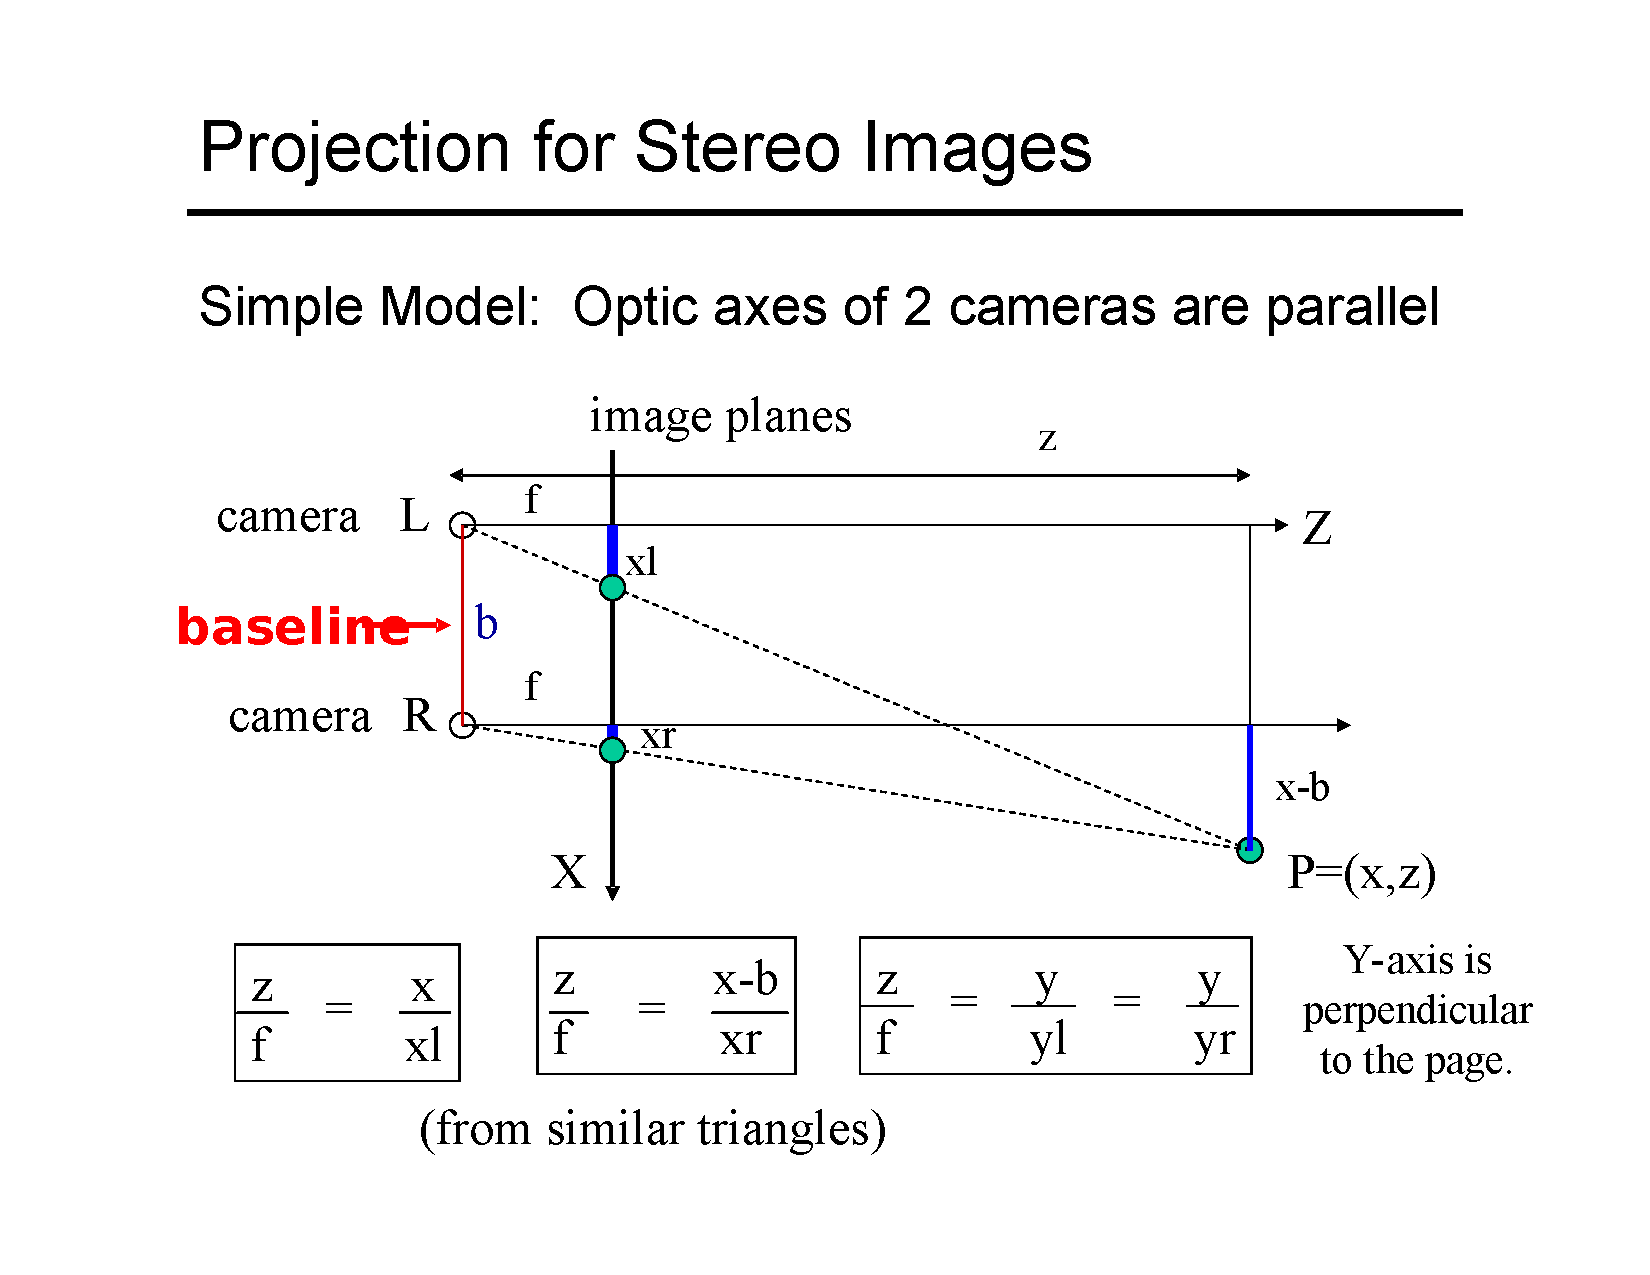
\includegraphics[width=0.8\linewidth]{lol.pdf}
\end{figure}
}
\only<2>{
By considering the two similar triangles, we can deduce the result of Disparity in the stereo images. This result is for one identical pixel of both the images. To find this identical pixel we use three different methods.
\begin{enumerate}
\item Cross correlation or SSD using small windows(Batch).
\item Symbolic feature matching, usually using segments/corners.
\item Use the newer interest operators, e.g., SIFT.
\end{enumerate}
}
\only<3>{
\begin{block}{Epipolar Constraint for Correspondence}
A plane is drawn joining the points \textbf{P} and camera \textbf{L} and \textbf{R} is called as Epipolar plane. This Epipolar plane cuts through image planes forming an epipolar line in each plane. We use this line to search for similar pixels in the two images rather than searching all the images.
\end{block}
\begin{figure}
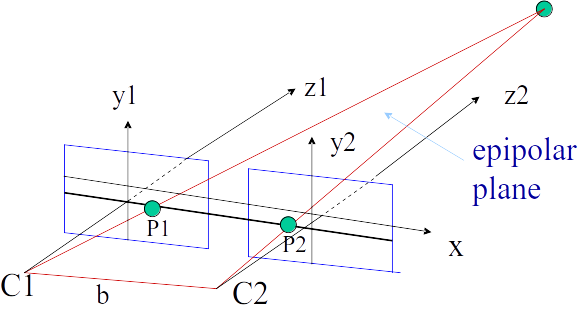
\includegraphics[width=0.7\linewidth]{epipolar_plane.png}
\end{figure}
}
\end{frame}

%------------------------------------------------

\begin{frame}
\frametitle{Implementation}
The Implementation of this concept is done in python. The database used is from this \href{http://vision.middlebury.edu/stereo/data/}{link}. A straight forward implemenntation is done, after which results are saved. The block size used is 8. Some filtering is also done to make the image clear.
\end{frame}

%------------------------------------------------

\begin{frame}[shrink=20]
\frametitle{Program}
\verbatiminput{program.py}
\end{frame}

%------------------------------------------------

\begin{frame}
\frametitle{Implementation}
The Implementation of this concept is done in python. The database used is from this \href{http://vision.middlebury.edu/stereo/data/}{link}. A straight forward implemenntation is done, after which results are saved. The block size used is 8. Some filtering is also done to make the image clear.
\end{frame}

%------------------------------------------------

\begin{frame}
\frametitle{Results}
Aloe
\begin{columns}[c] % The "c" option specifies centered vertical alignment while the "t" option is used for top vertical alignment

\column{.45\textwidth} % Left column and width
\begin{figure}
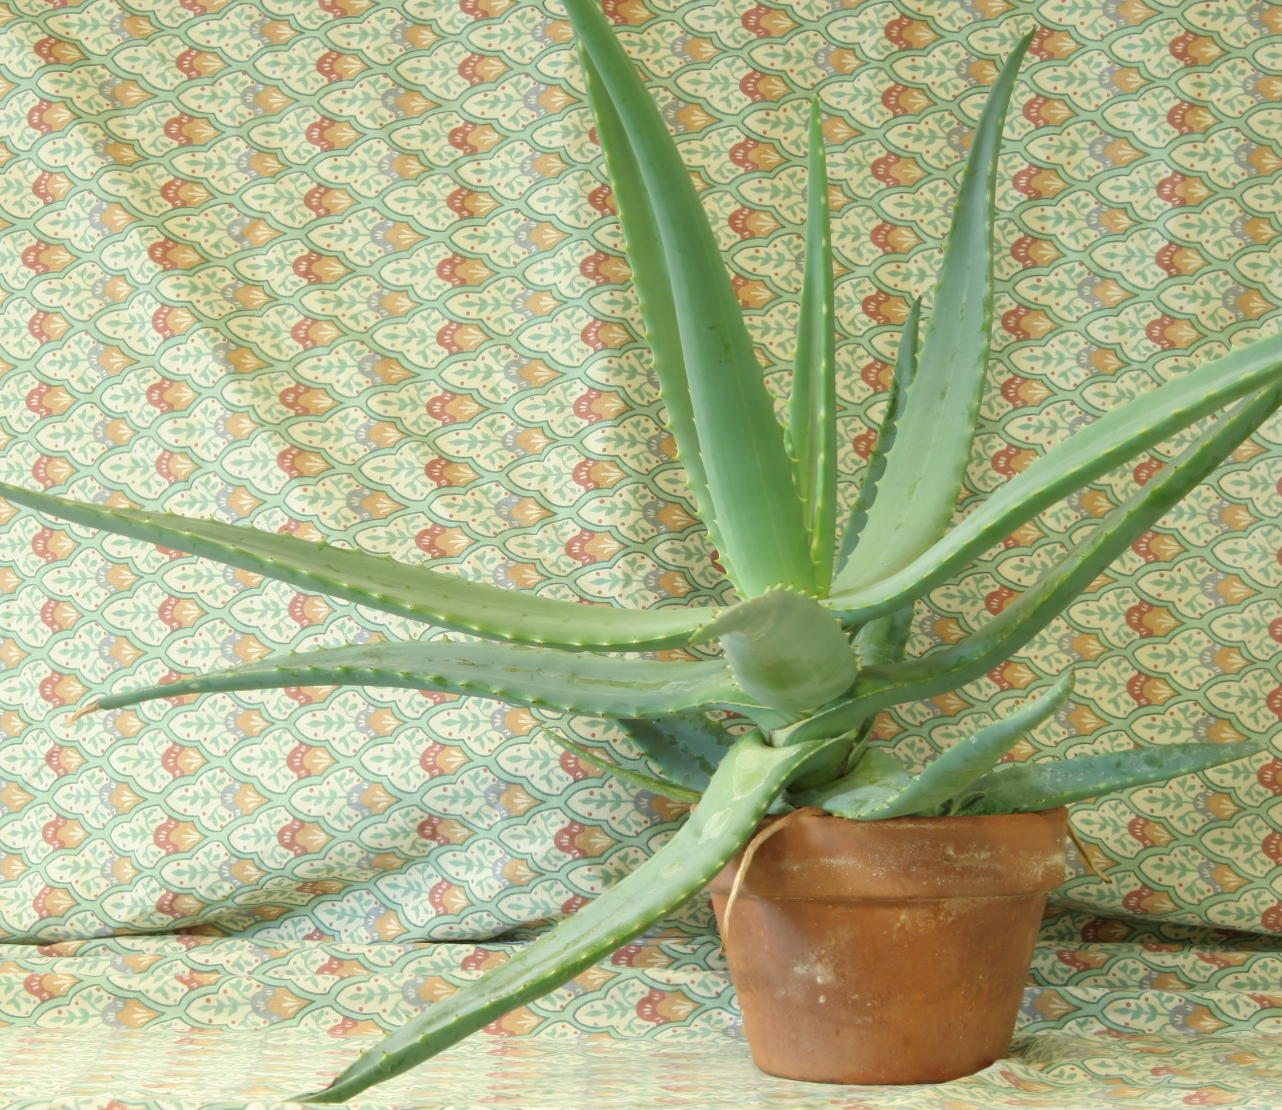
\includegraphics[width=0.7\linewidth]{../program/dataset/Aloe/view1.png}
\end{figure}

\column{.5\textwidth} % Right column and width
\begin{figure}
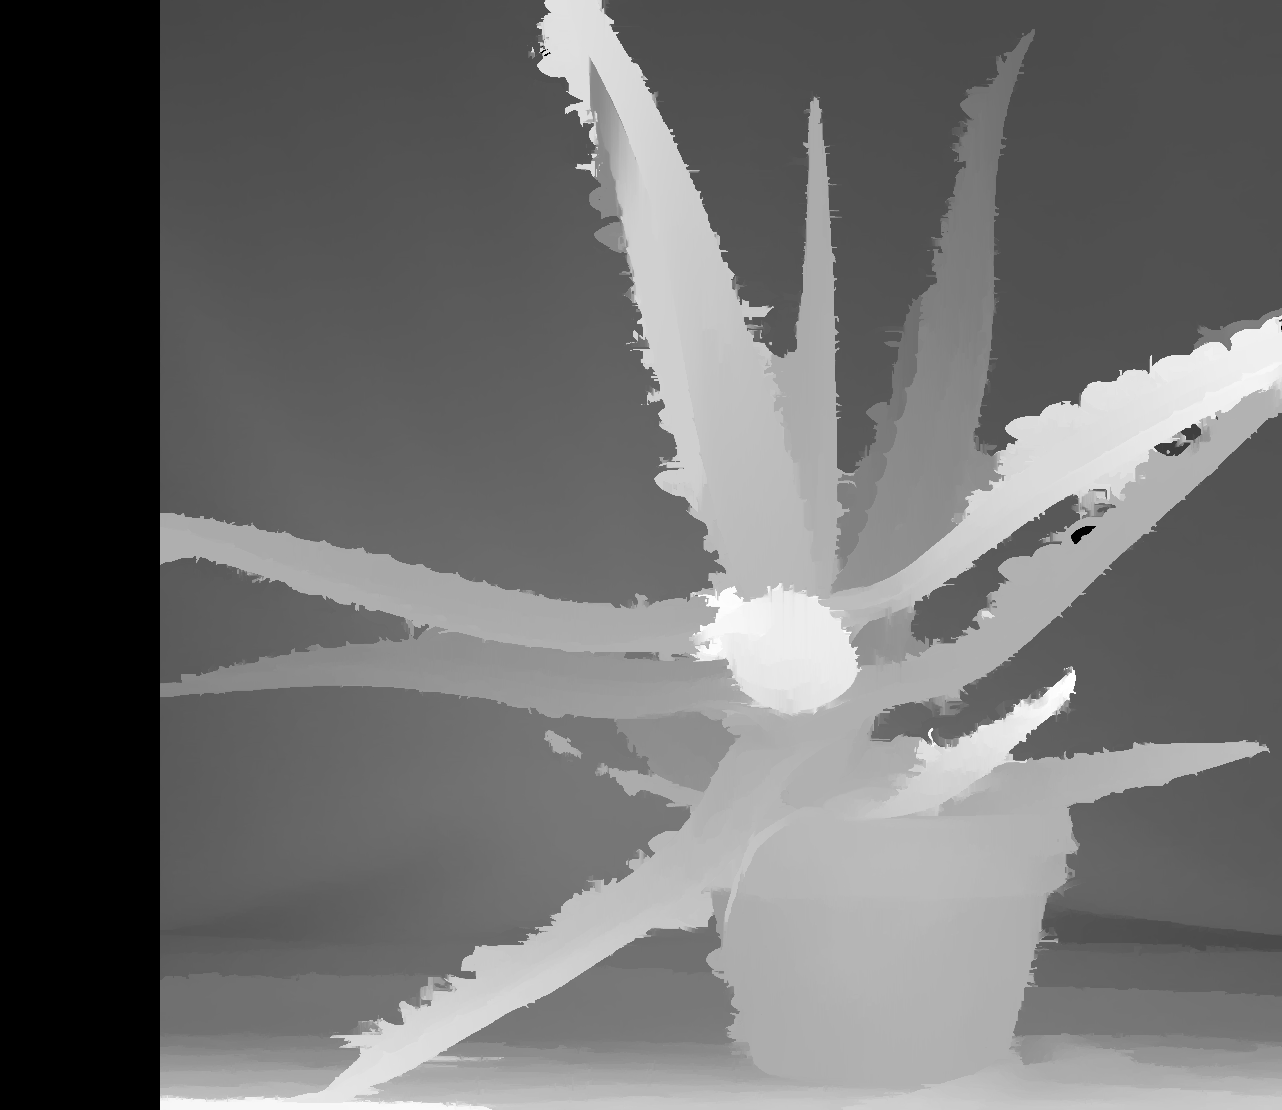
\includegraphics[width=0.7\linewidth]{../program/Result/Aloe.png}
\end{figure}

\end{columns}
\end{frame}

%------------------------------------------------

\begin{frame}
\frametitle{Results}
Baby1
\begin{columns}[c] % The "c" option specifies centered vertical alignment while the "t" option is used for top vertical alignment

\column{.45\textwidth} % Left column and width
\begin{figure}
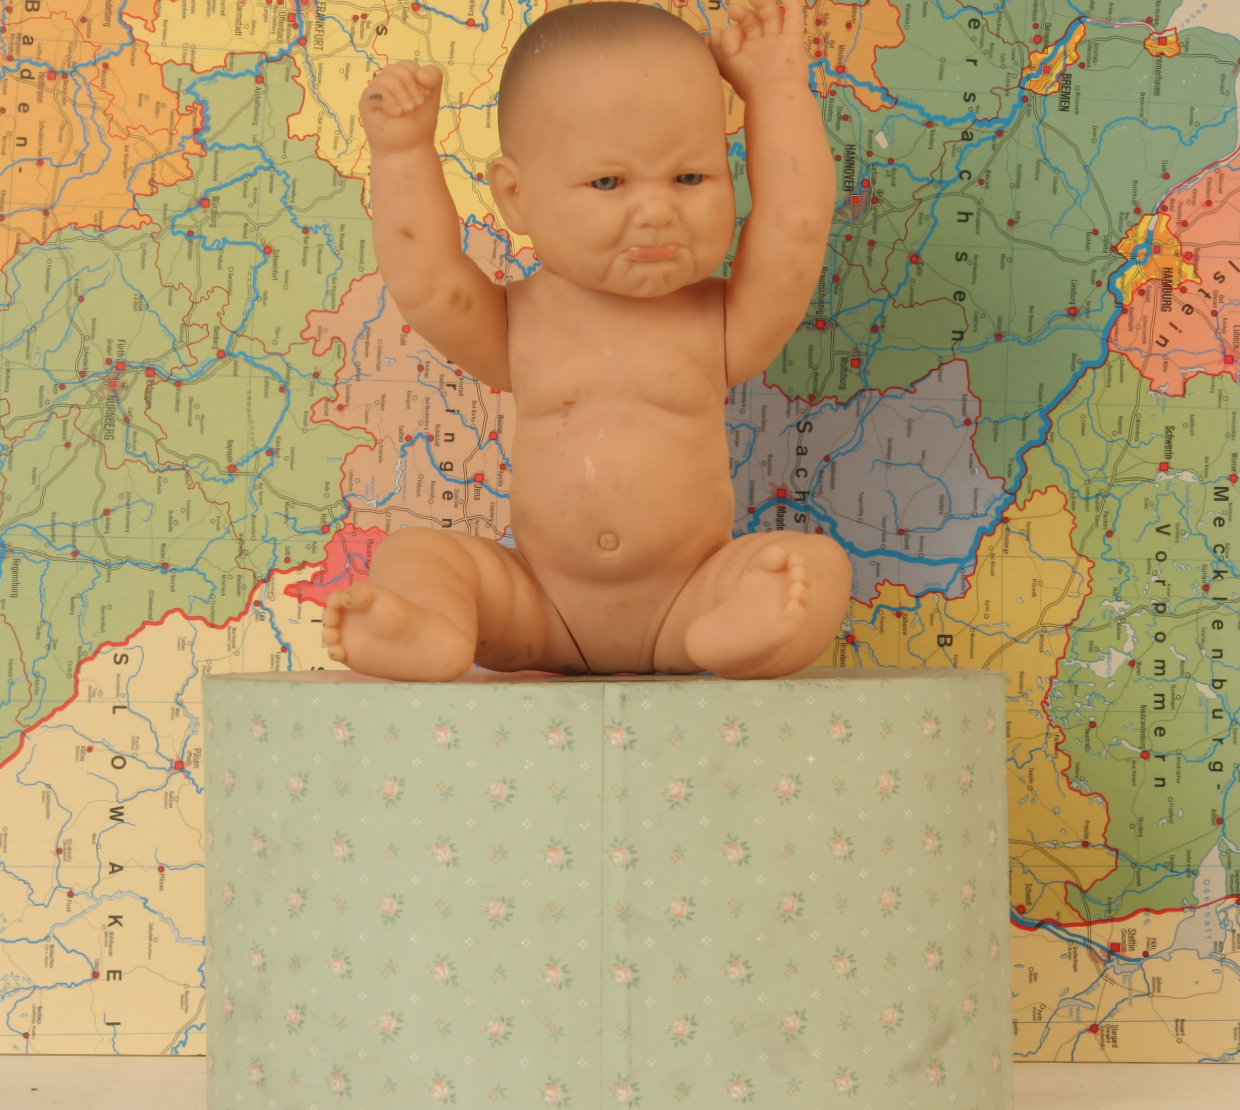
\includegraphics[width=0.7\linewidth]{../program/dataset/Baby1/view1.png}
\end{figure}

\column{.5\textwidth} % Right column and width
\begin{figure}
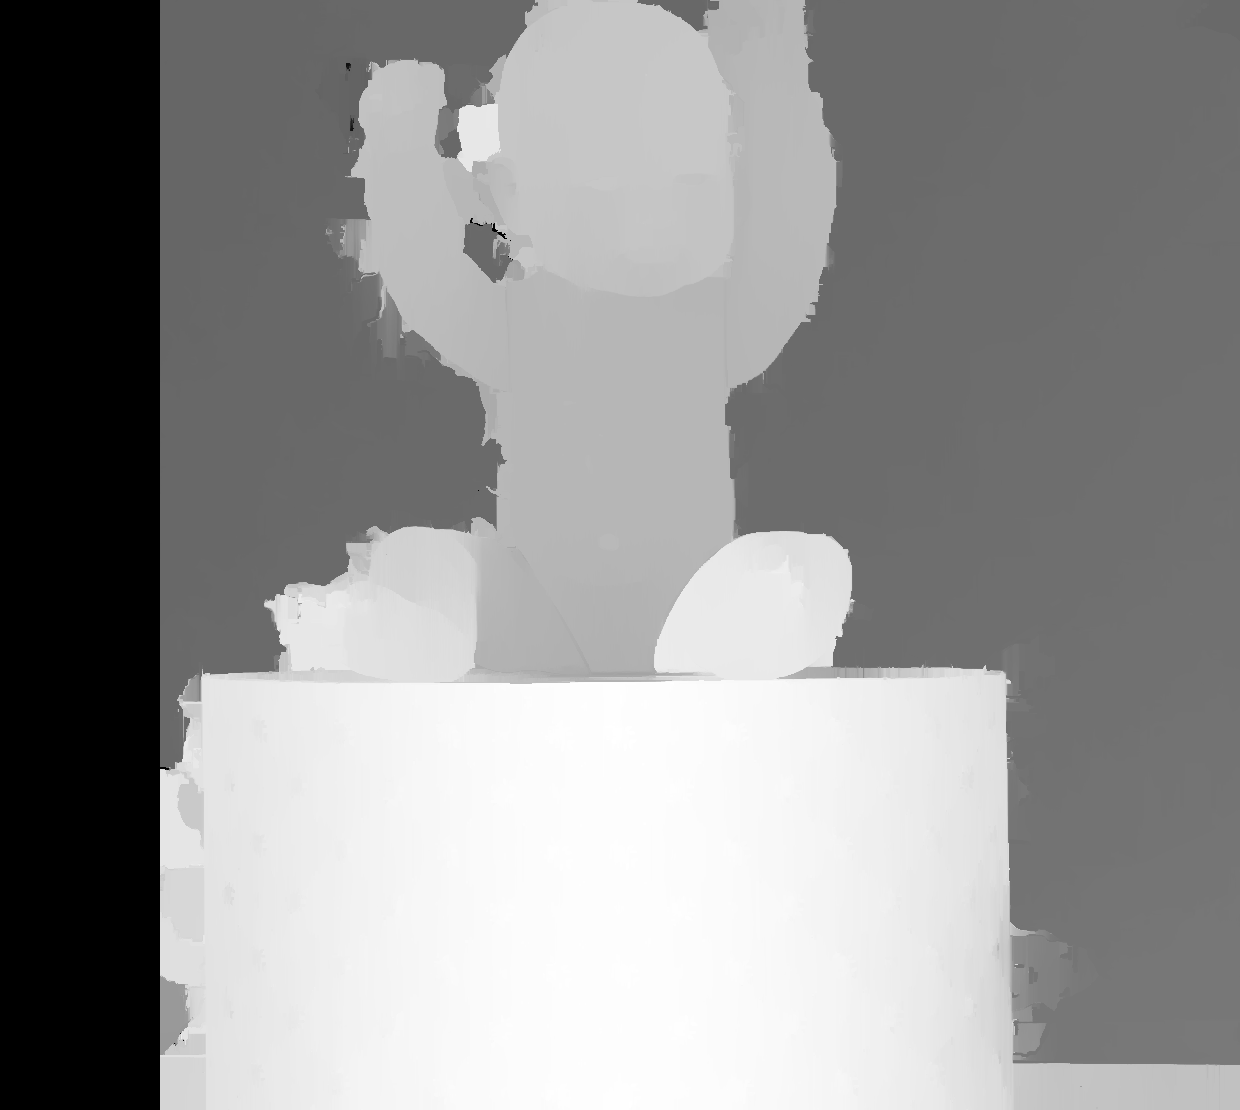
\includegraphics[width=0.7\linewidth]{../program/Result/Baby1.png}
\end{figure}

\end{columns}
\end{frame}

%------------------------------------------------

\begin{frame}
\frametitle{Results}
Cloth1
\begin{columns}[c] % The "c" option specifies centered vertical alignment while the "t" option is used for top vertical alignment

\column{.45\textwidth} % Left column and width
\begin{figure}
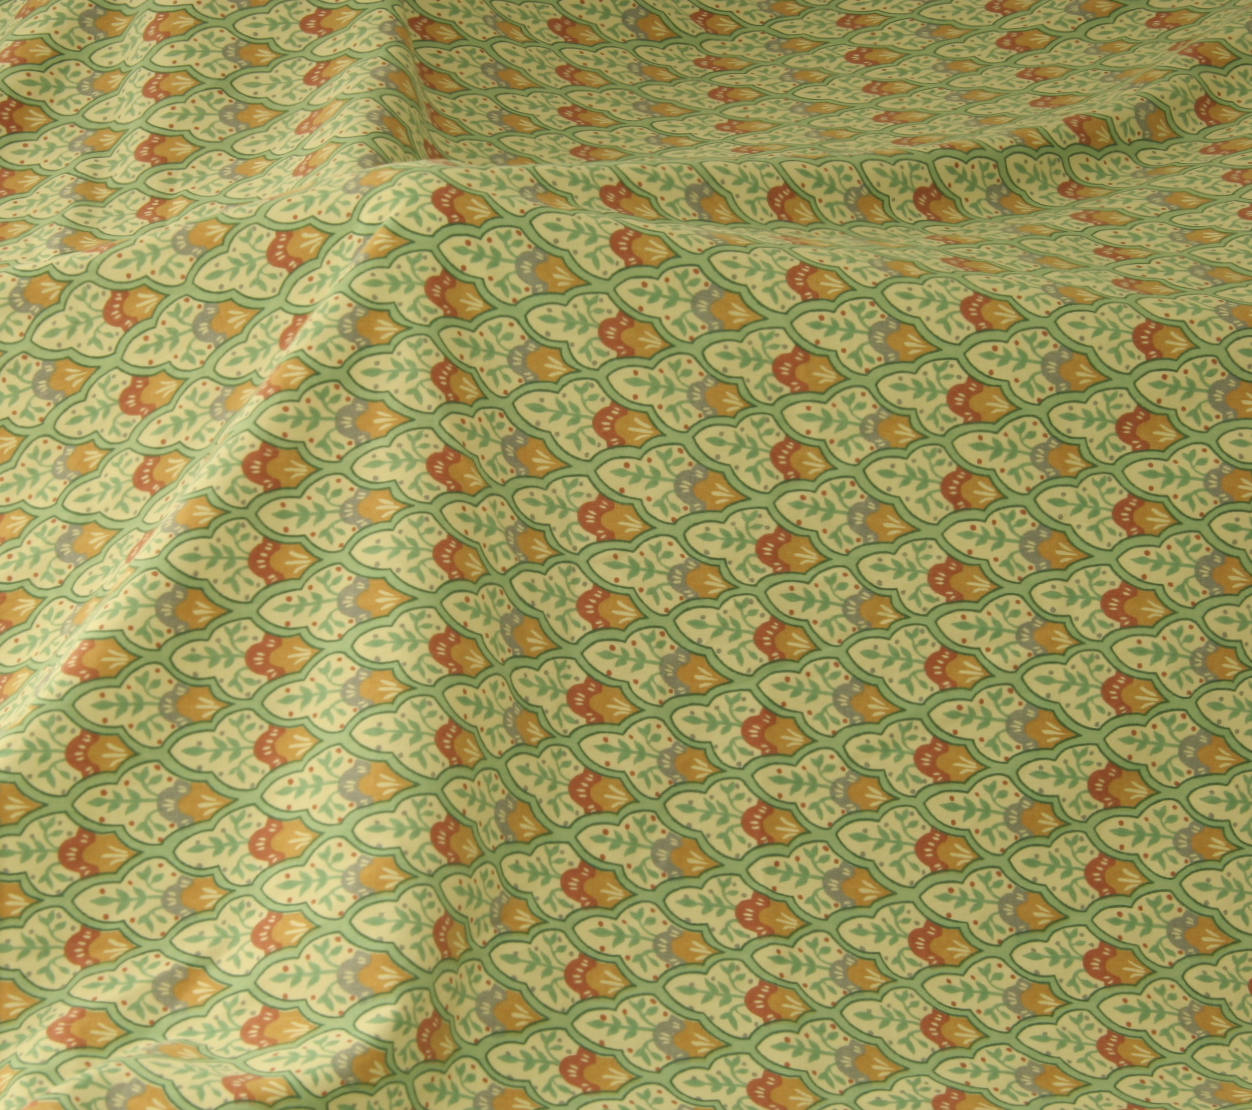
\includegraphics[width=0.7\linewidth]{../program/dataset/Cloth1/view1.png}
\end{figure}

\column{.5\textwidth} % Right column and width
\begin{figure}
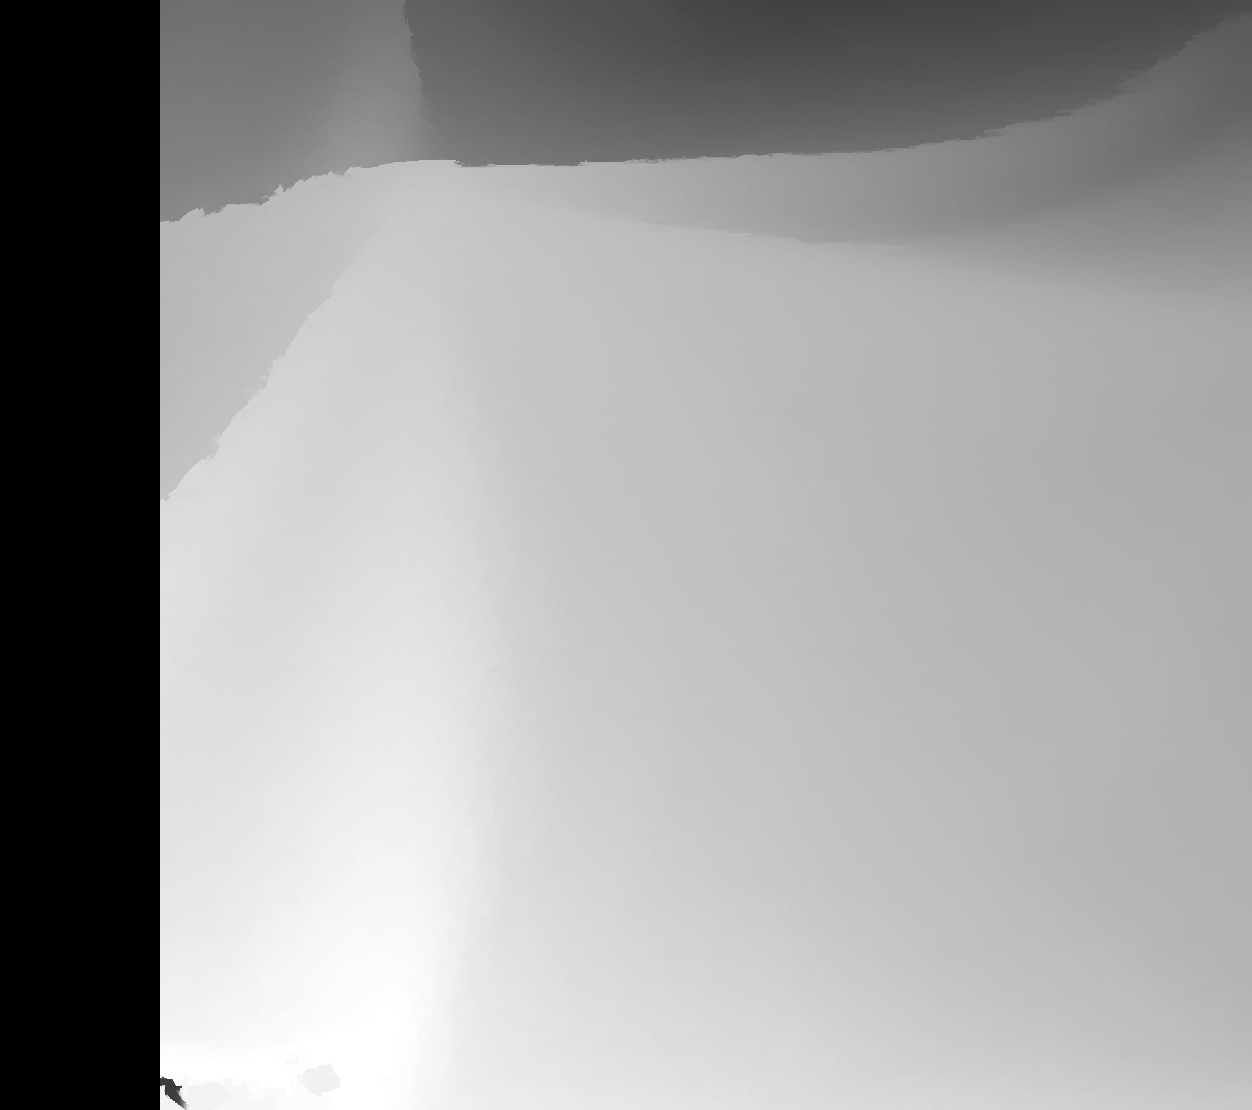
\includegraphics[width=0.7\linewidth]{../program/Result/Cloth1.png}
\end{figure}

\end{columns}
\end{frame}

%------------------------------------------------

\begin{frame}
\frametitle{Results}
Lampshade1
\begin{columns}[c] % The "c" option specifies centered vertical alignment while the "t" option is used for top vertical alignment

\column{.45\textwidth} % Left column and width
\begin{figure}
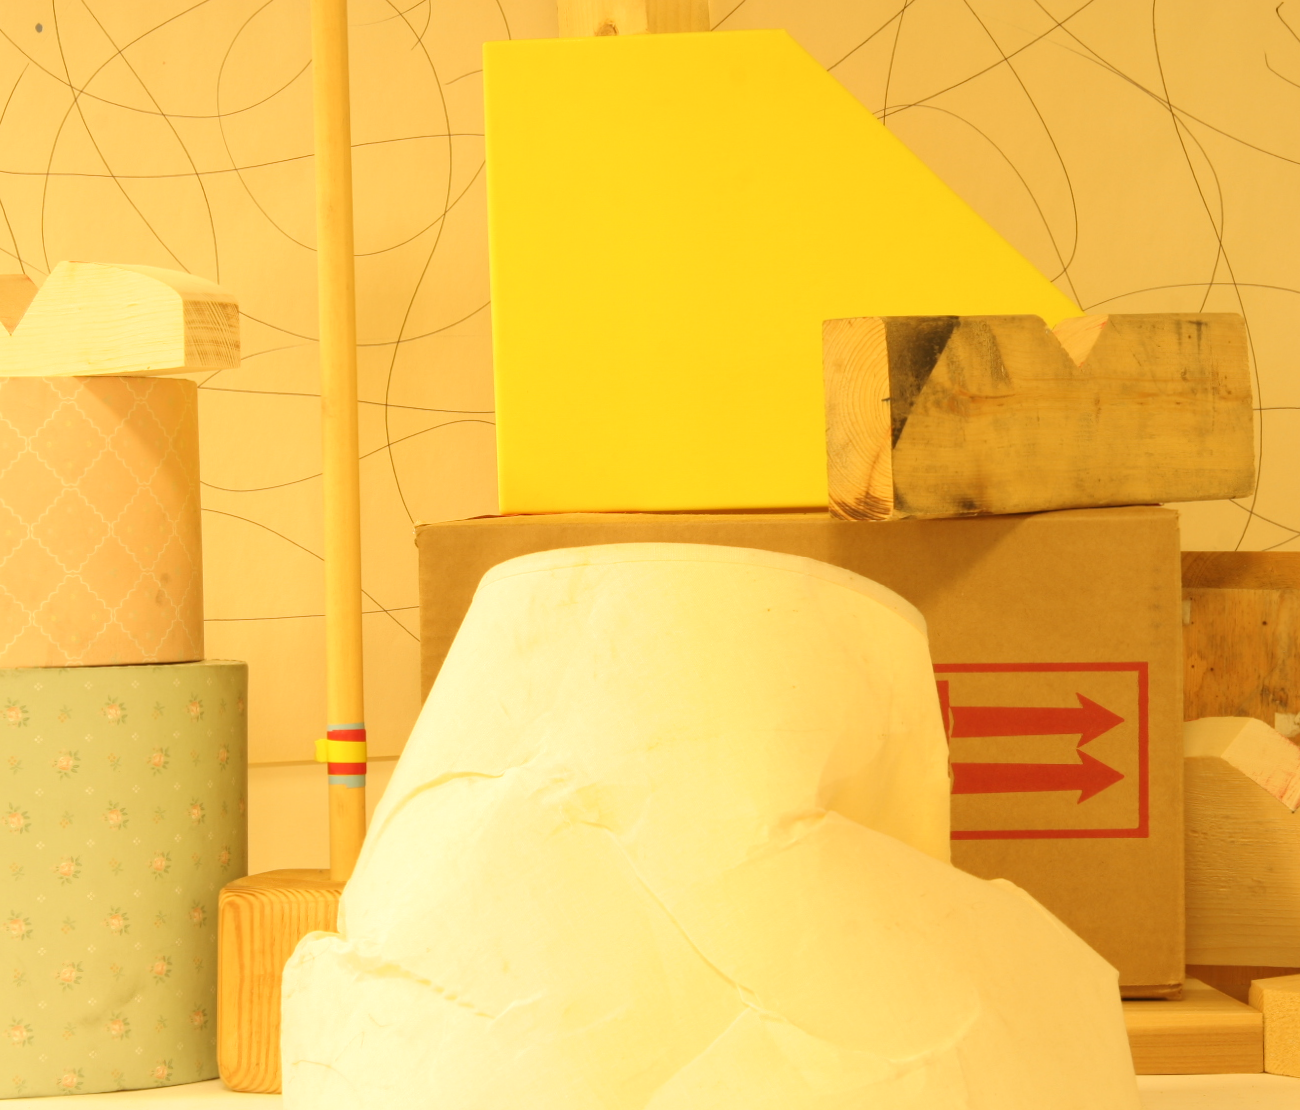
\includegraphics[width=0.7\linewidth]{../program/dataset/Lampshade1/view1.png}
\end{figure}

\column{.5\textwidth} % Right column and width
\begin{figure}
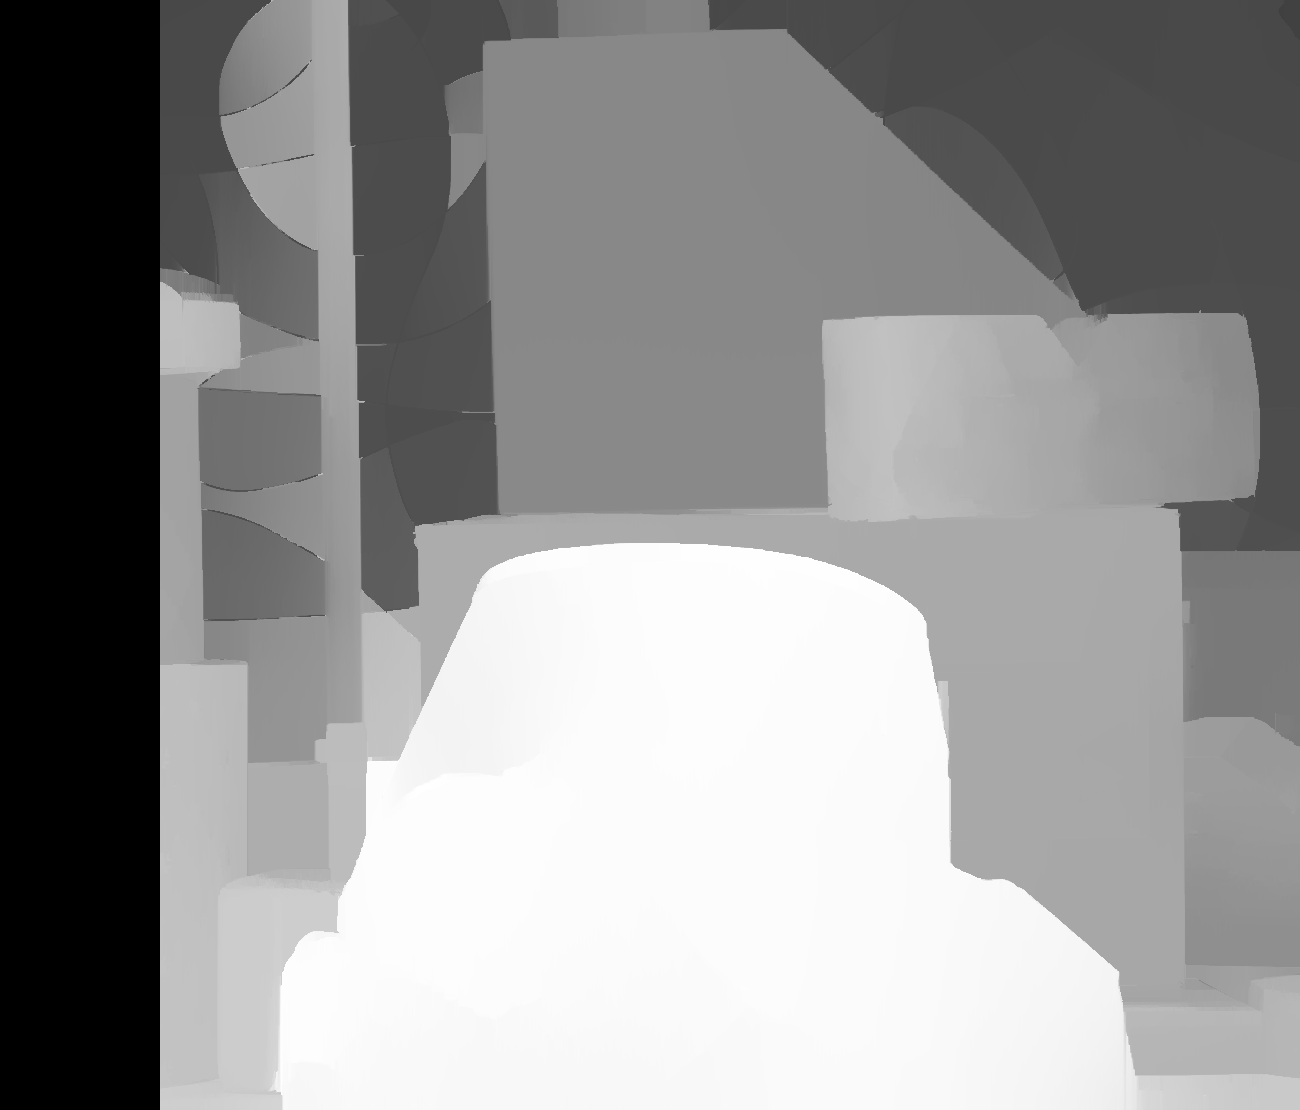
\includegraphics[width=0.7\linewidth]{../program/Result/Lampshade1.png}
\end{figure}

\end{columns}
\end{frame}

%------------------------------------------------

\begin{frame}
\frametitle{Results}
Midd1
\begin{columns}[c] % The "c" option specifies centered vertical alignment while the "t" option is used for top vertical alignment

\column{.45\textwidth} % Left column and width
\begin{figure}
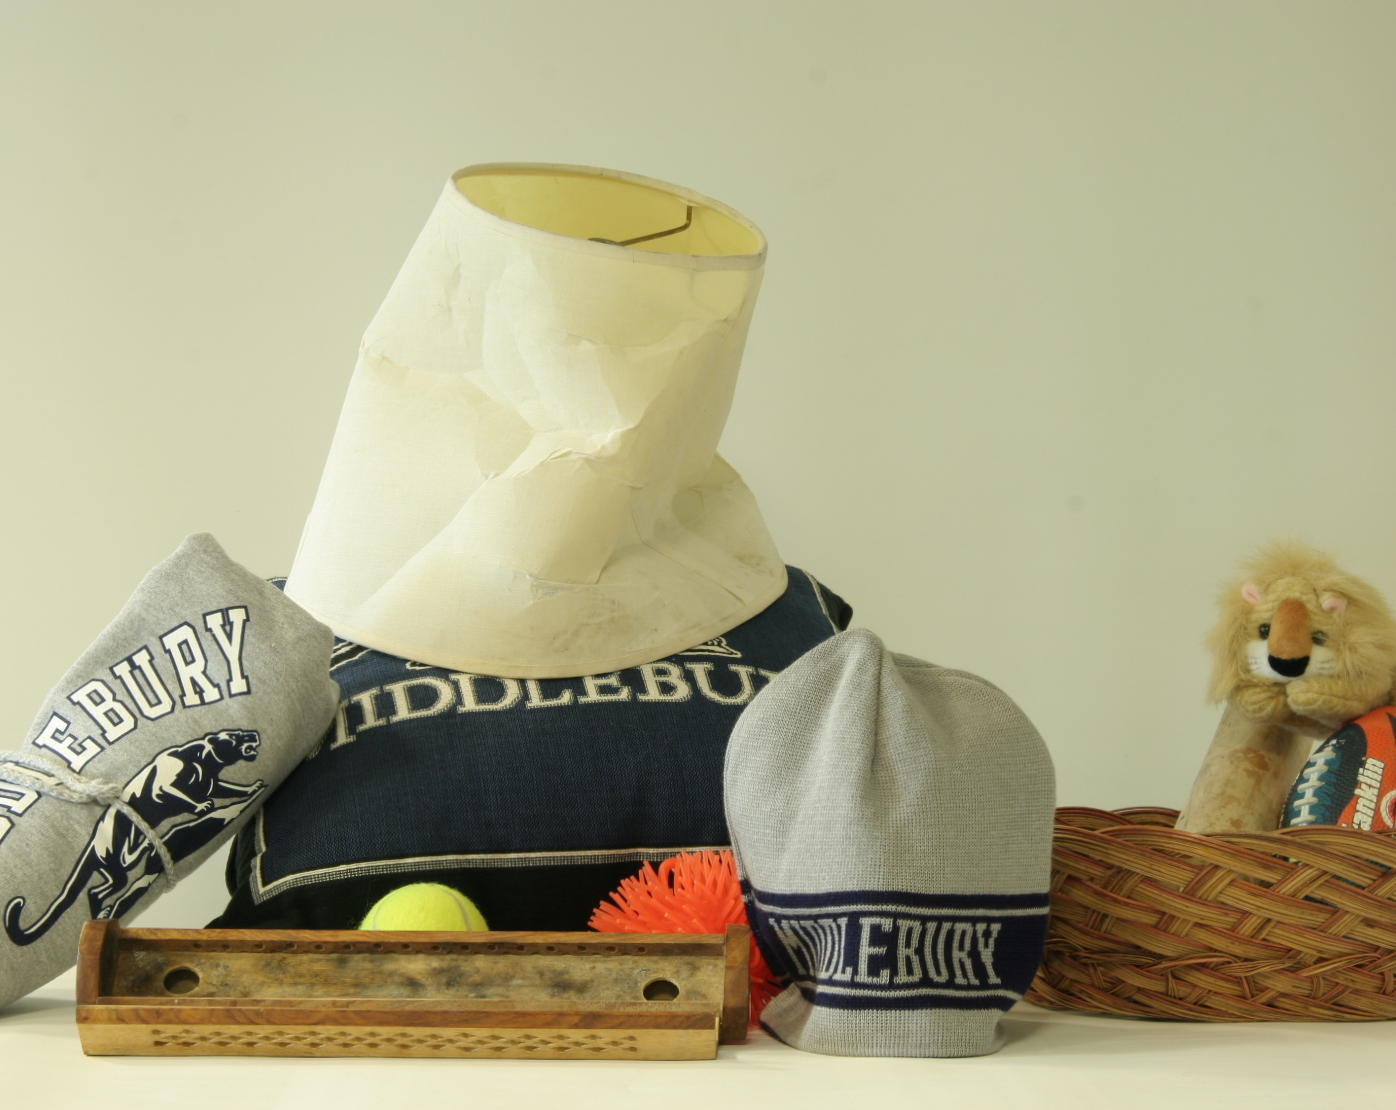
\includegraphics[width=0.7\linewidth]{../program/dataset/Midd1/view1.png}
\end{figure}

\column{.5\textwidth} % Right column and width
\begin{figure}
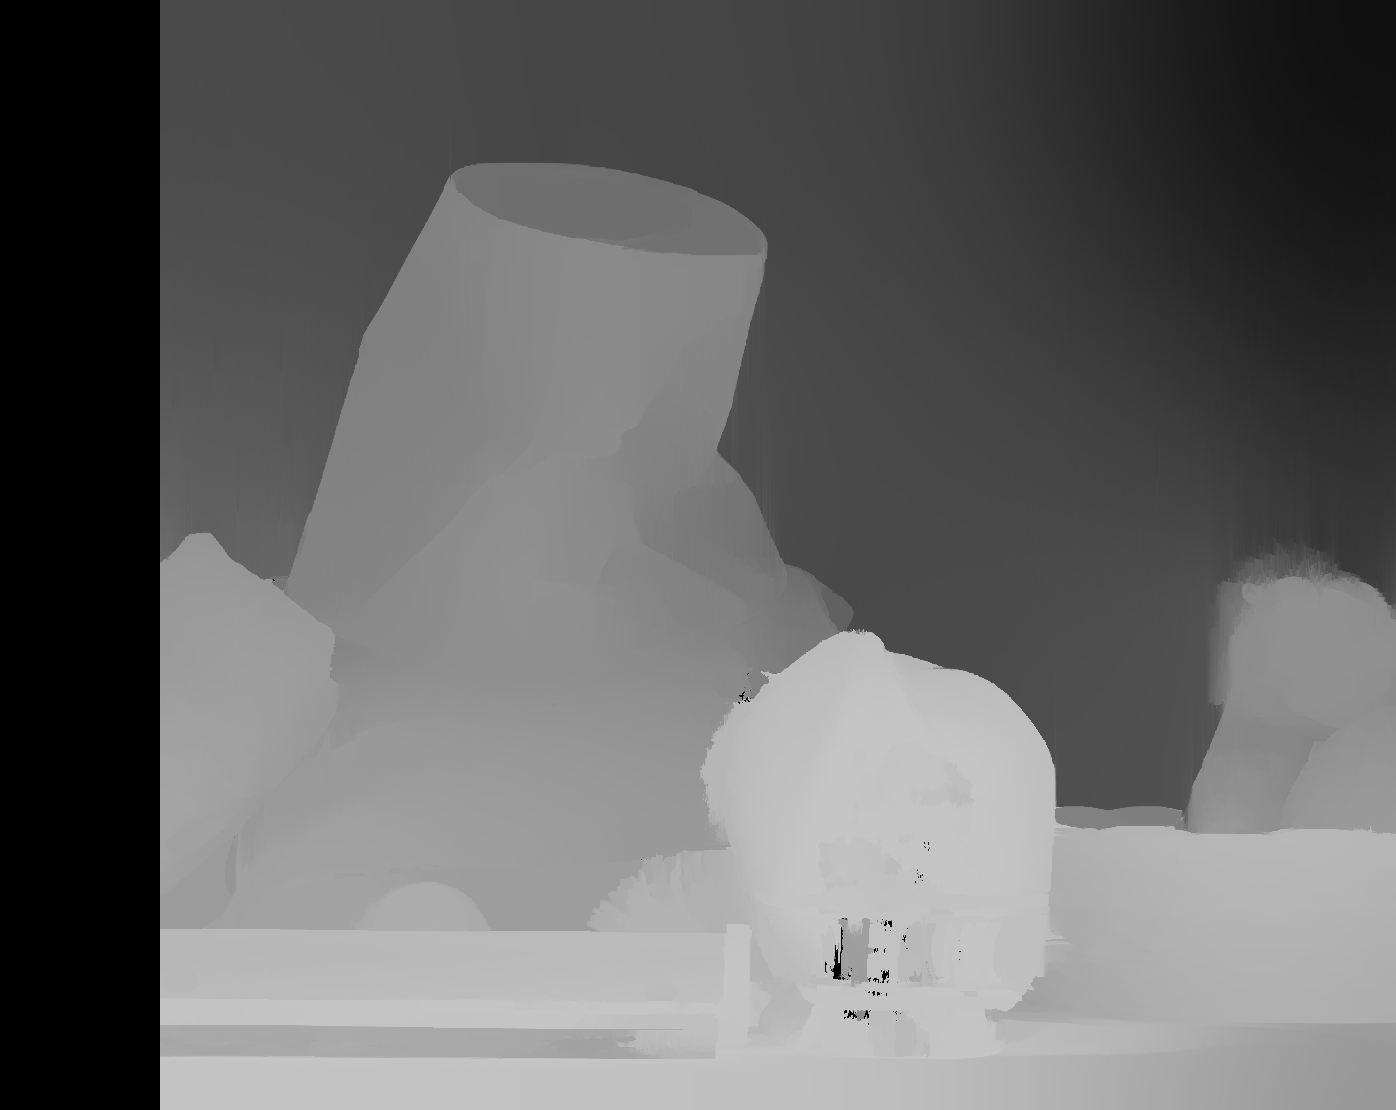
\includegraphics[width=0.7\linewidth]{../program/Result/Midd1.png}
\end{figure}

\end{columns}
\end{frame}

%------------------------------------------------

\begin{frame}
\frametitle{Results}
Plastic
\begin{columns}[c] % The "c" option specifies centered vertical alignment while the "t" option is used for top vertical alignment

\column{.45\textwidth} % Left column and width
\begin{figure}
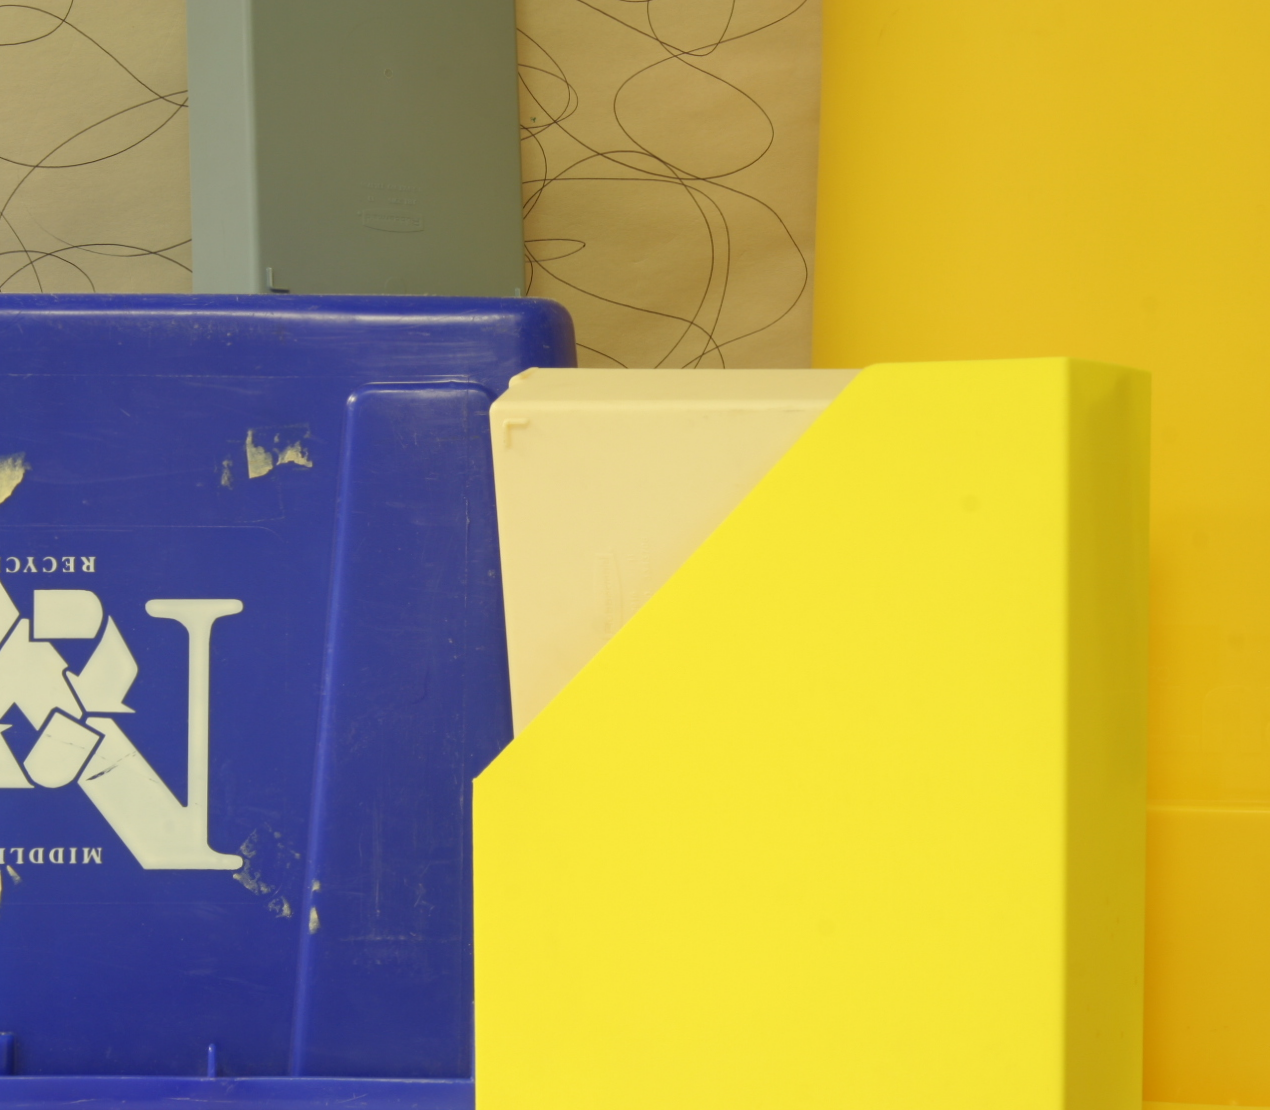
\includegraphics[width=0.7\linewidth]{../program/dataset/Plastic/view1.png}
\end{figure}

\column{.5\textwidth} % Right column and width
\begin{figure}
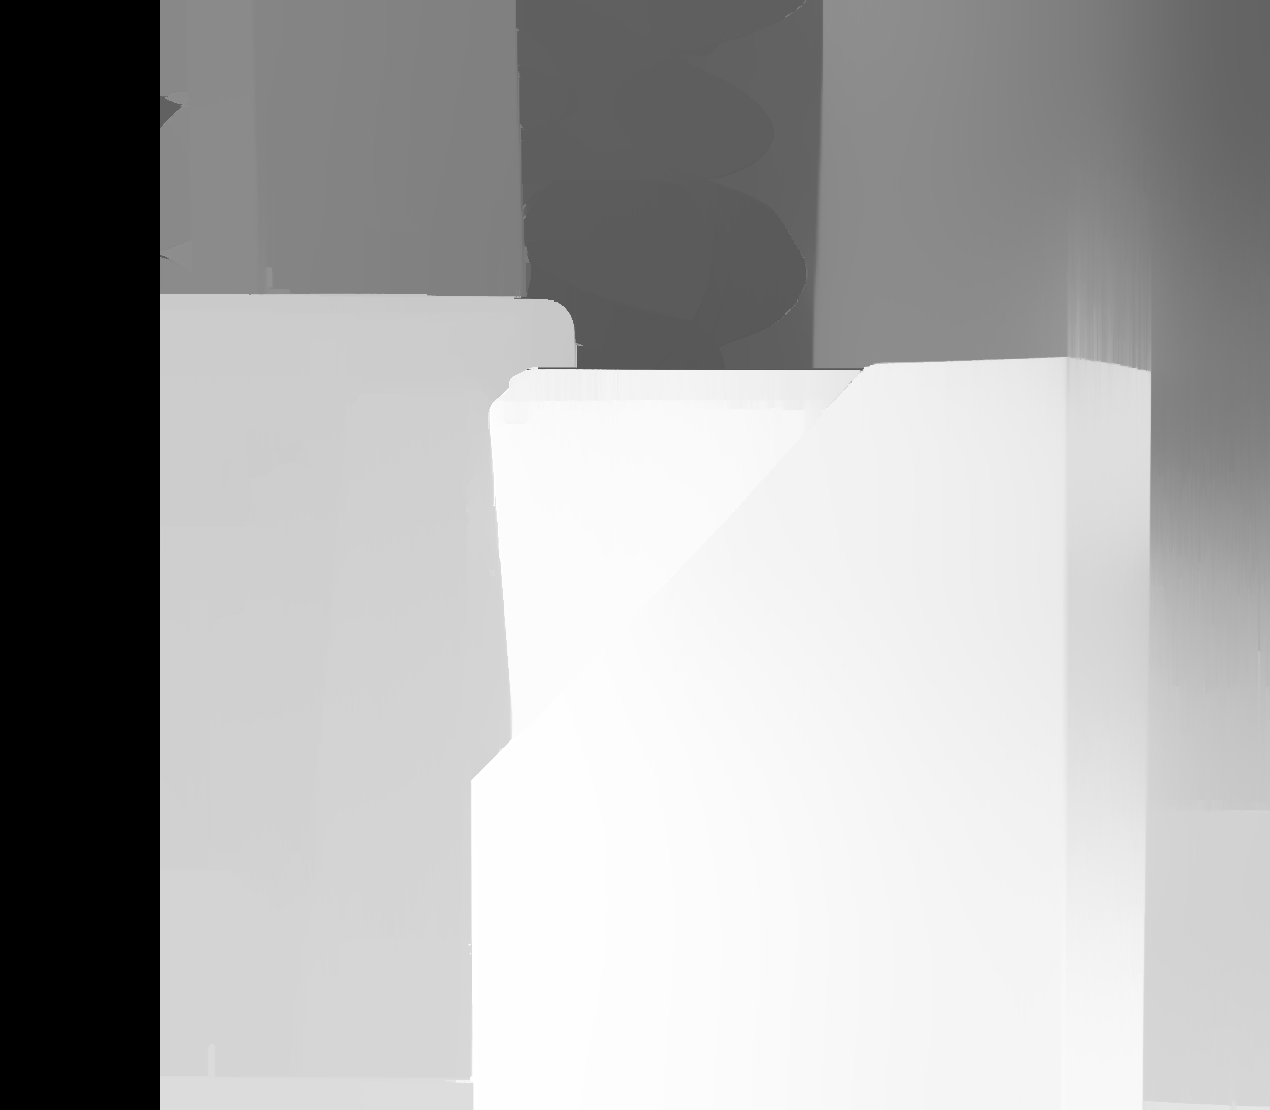
\includegraphics[width=0.7\linewidth]{../program/Result/Plastic.png}
\end{figure}

\end{columns}
\end{frame}

%------------------------------------------------

\begin{frame}
\frametitle{Results}
Rocks1
\begin{columns}[c] % The "c" option specifies centered vertical alignment while the "t" option is used for top vertical alignment

\column{.45\textwidth} % Left column and width
\begin{figure}
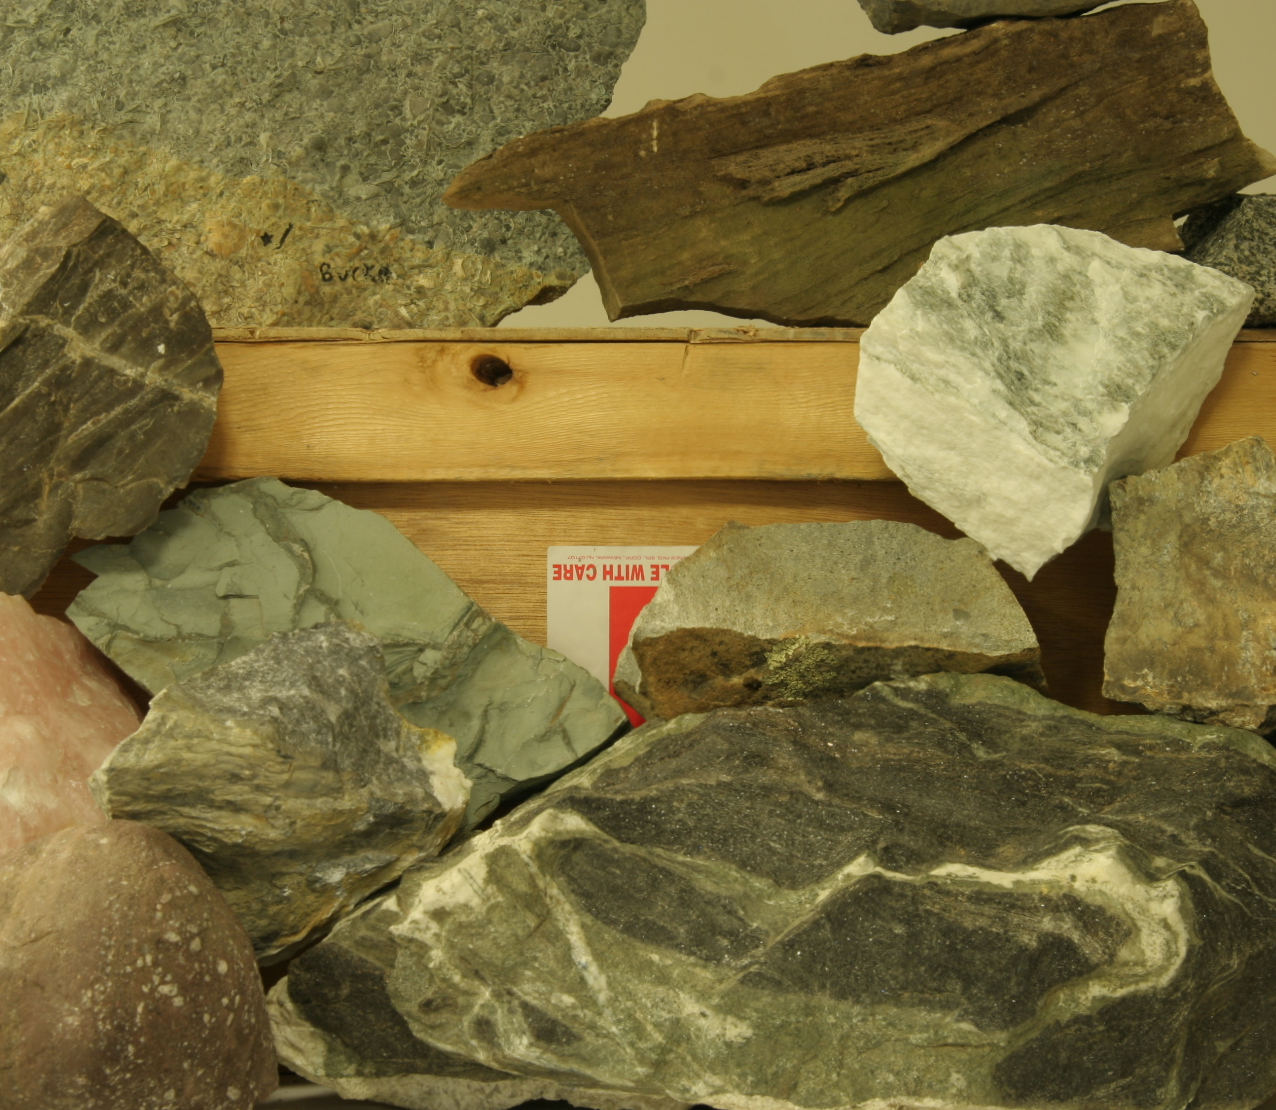
\includegraphics[width=0.7\linewidth]{../program/dataset/Rocks1/view1.png}
\end{figure}

\column{.5\textwidth} % Right column and width
\begin{figure}
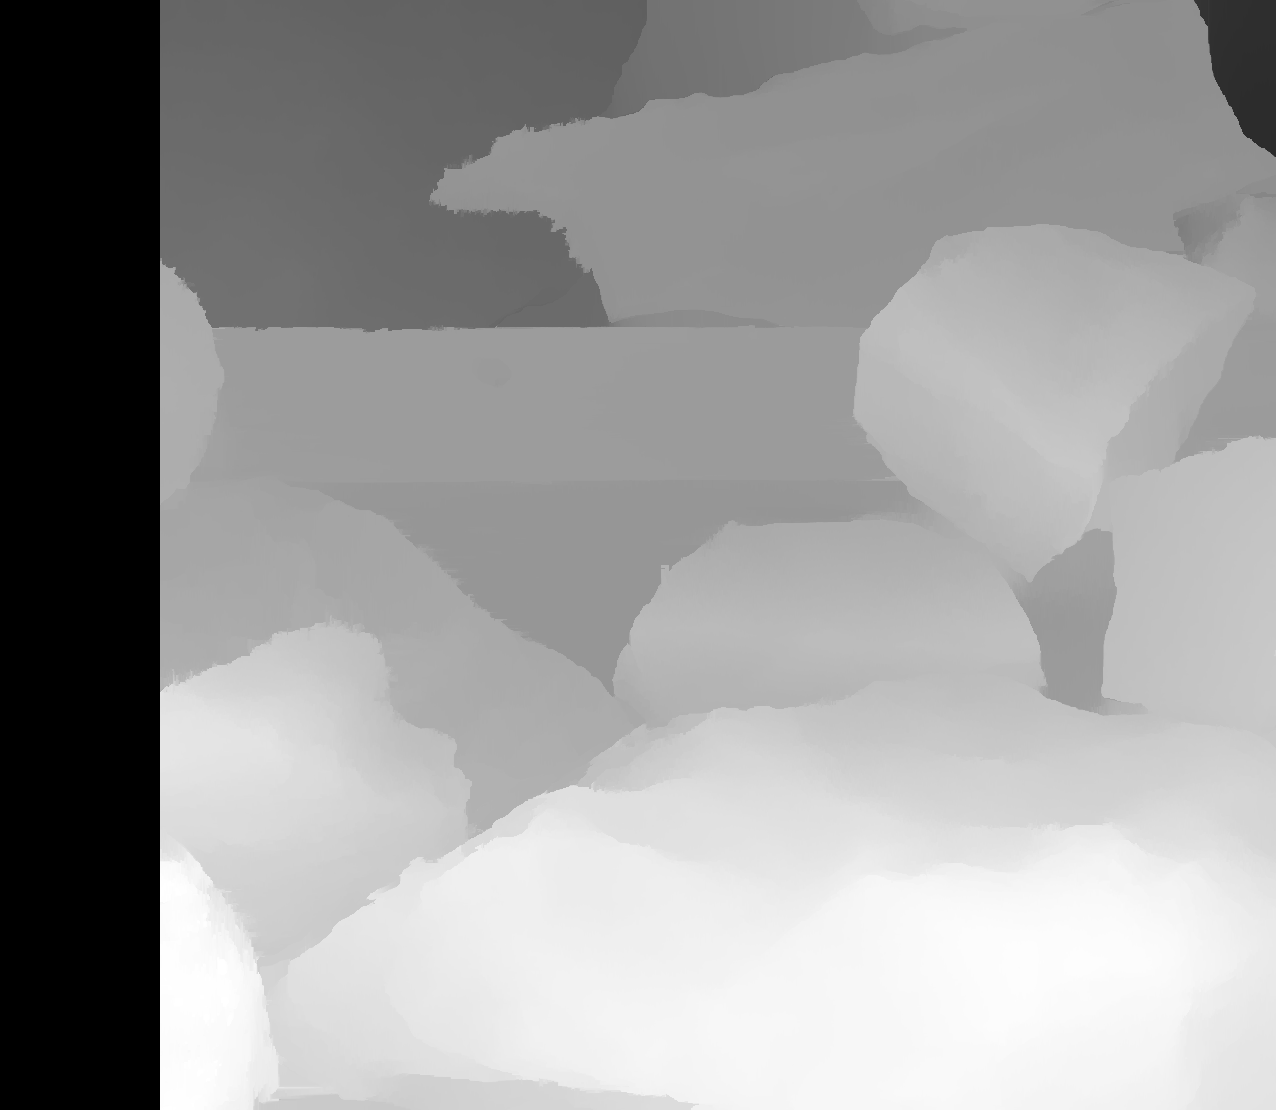
\includegraphics[width=0.7\linewidth]{../program/Result/Rocks1.png}
\end{figure}

\end{columns}
\end{frame}

%------------------------------------------------

\begin{frame}
\frametitle{Results}
Wood1
\begin{columns}[c] % The "c" option specifies centered vertical alignment while the "t" option is used for top vertical alignment

\column{.45\textwidth} % Left column and width
\begin{figure}
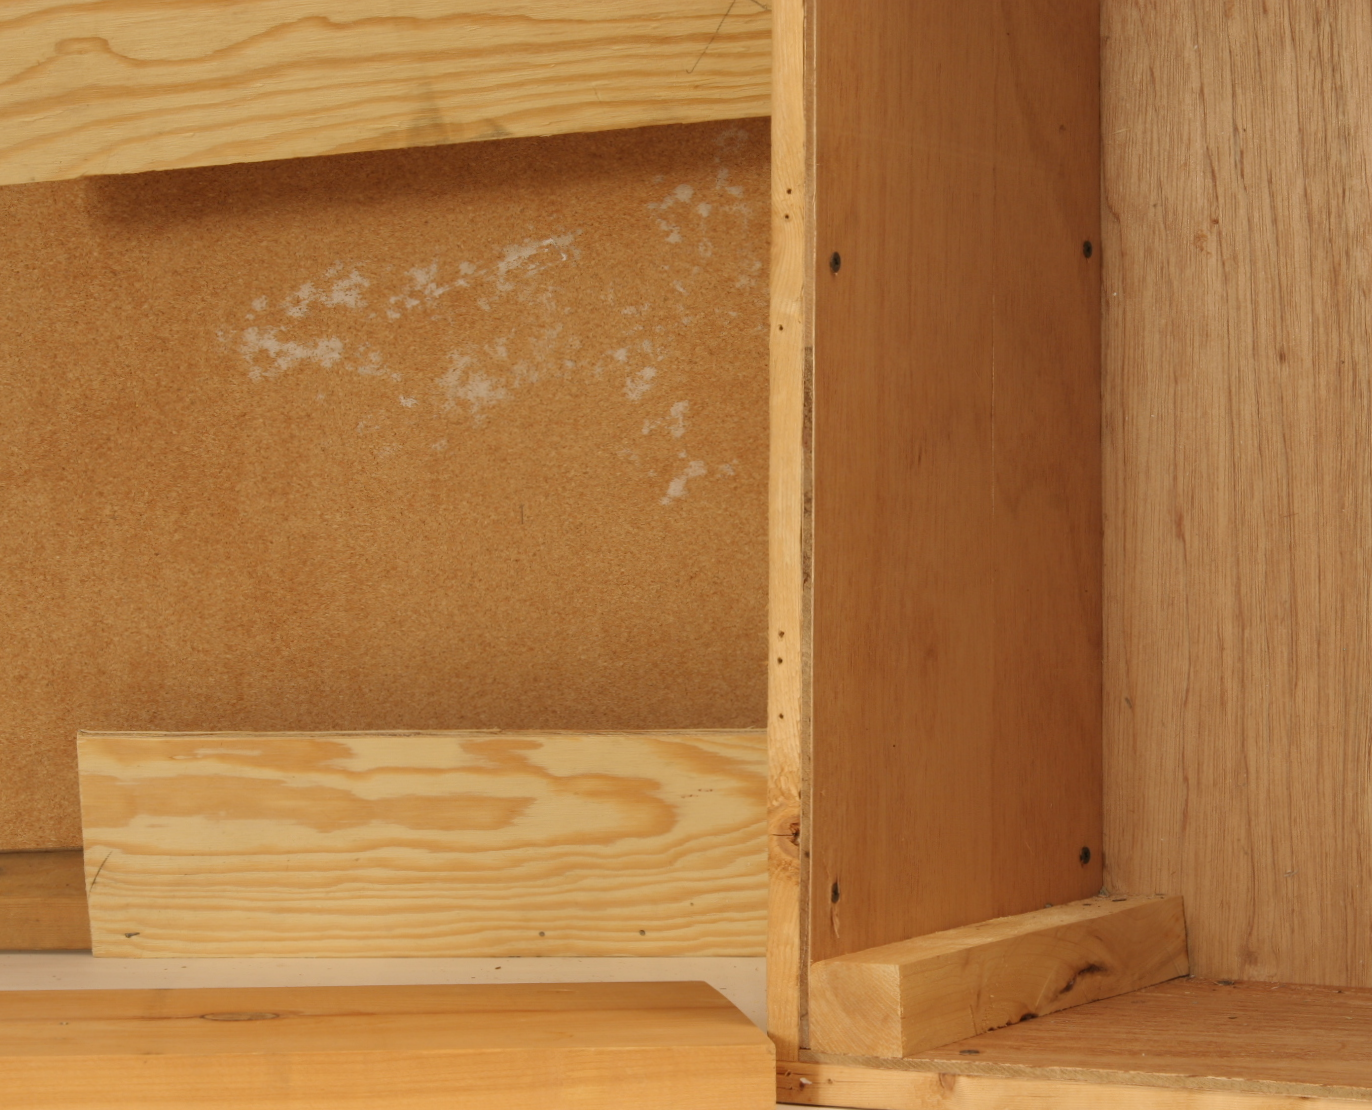
\includegraphics[width=0.7\linewidth]{../program/dataset/Wood1/view1.png}
\end{figure}

\column{.5\textwidth} % Right column and width
\begin{figure}
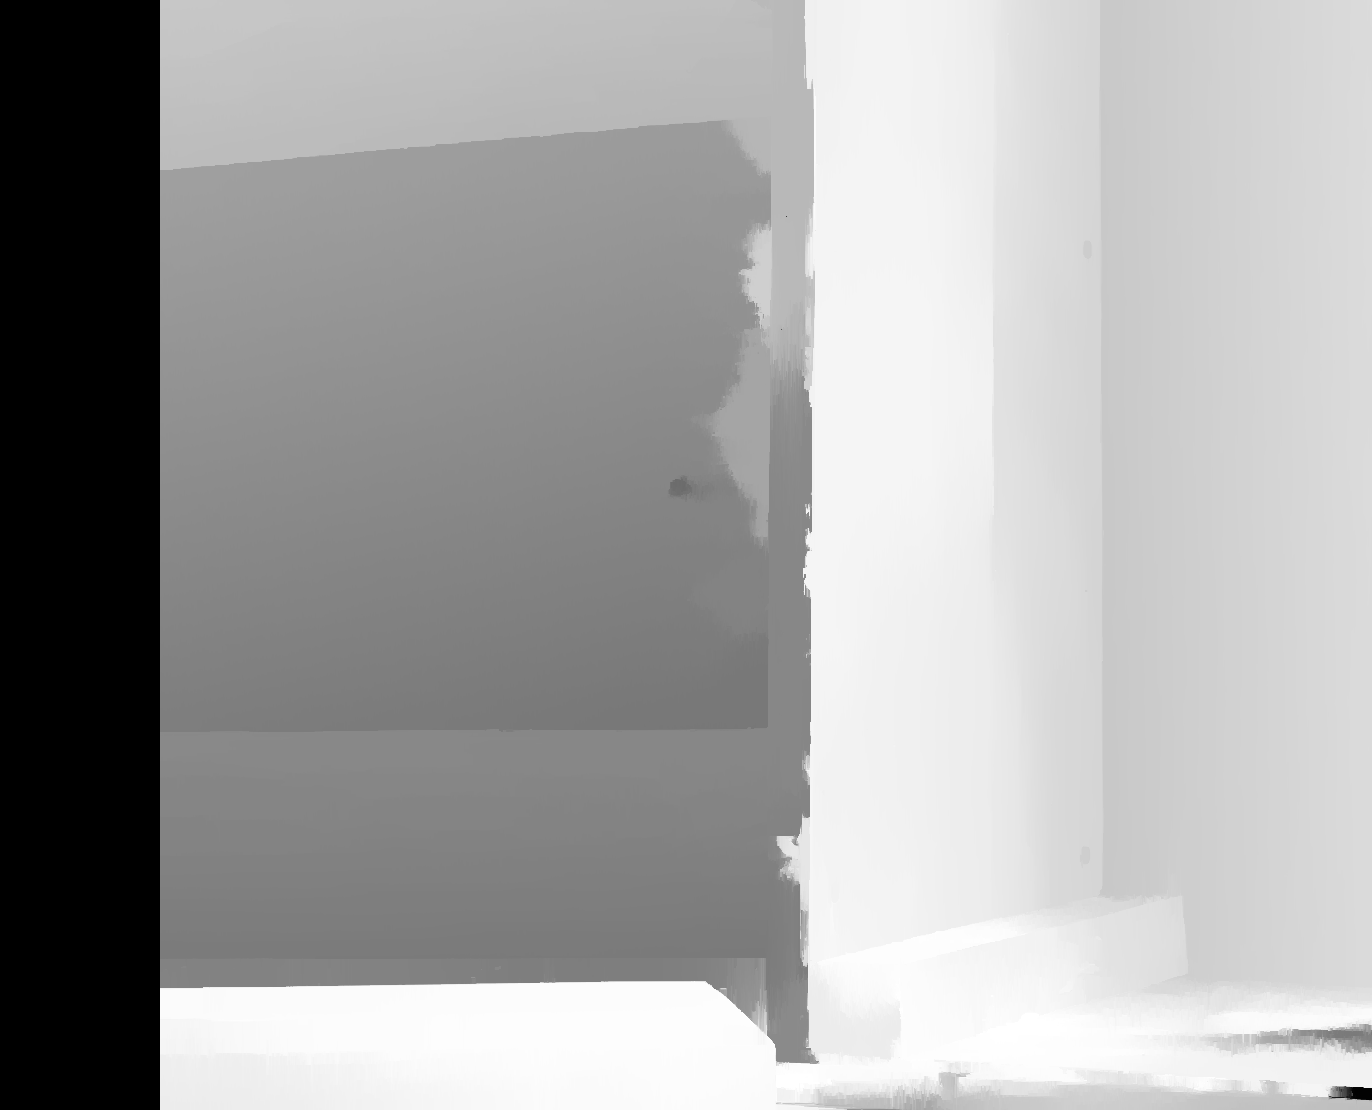
\includegraphics[width=0.7\linewidth]{../program/Result/Wood1.png}
\end{figure}

\end{columns}
\end{frame}


%------------------------------------------------

\begin{frame}
\frametitle{Things Learned}
From this assignment I have learned the theory behind Stereo Depth Estimation. A better and a clear understanding is achieved by implementing the same in python(using open-cv).
\end{frame}

%------------------------------------------------

\begin{frame}[shrink=5]
\frametitle{References}
\begin{itemize}
\item https://courses.cs.washington.edu/courses/cse455/09wi/Lects/lect16.pdf
\item http://www.cs.tut.fi/~suominen/SGN-1656-stereo/stereo\_instructions.pdf
\item http://vision.middlebury.edu/stereo/data/
\item http://timosam.com/python\_opencv\_depthimage
\end{itemize}
\end{frame}

%----------------------------------------------------------------------------------------

\end{document} 